\section{Cases Studies}

\subsection{Lazy Optimization vs. Better Fusion}
\label{ap:cases:profiling-lazy-optim}
We show the cases of profiling feedback from lazy optimization and better fusion cases. As shownin Figure~\ref{fig:profiling-lazy-optim}, in the lazy optimization case, where only a trivial summation operation is replaced, the model-generated kernel accounts for only $0.014\%$ of the total CUDA execution time. In contrast, with better fusion, the model generates more meaningful kernels, achieving significantly better speedup and increasing the CUDA runtime fraction to $86.15\%$ of the total runtime.
\begin{figure*}[htbp]
  \centering
  \begin{minipage}[t]{0.9\textwidth}
    \centering
    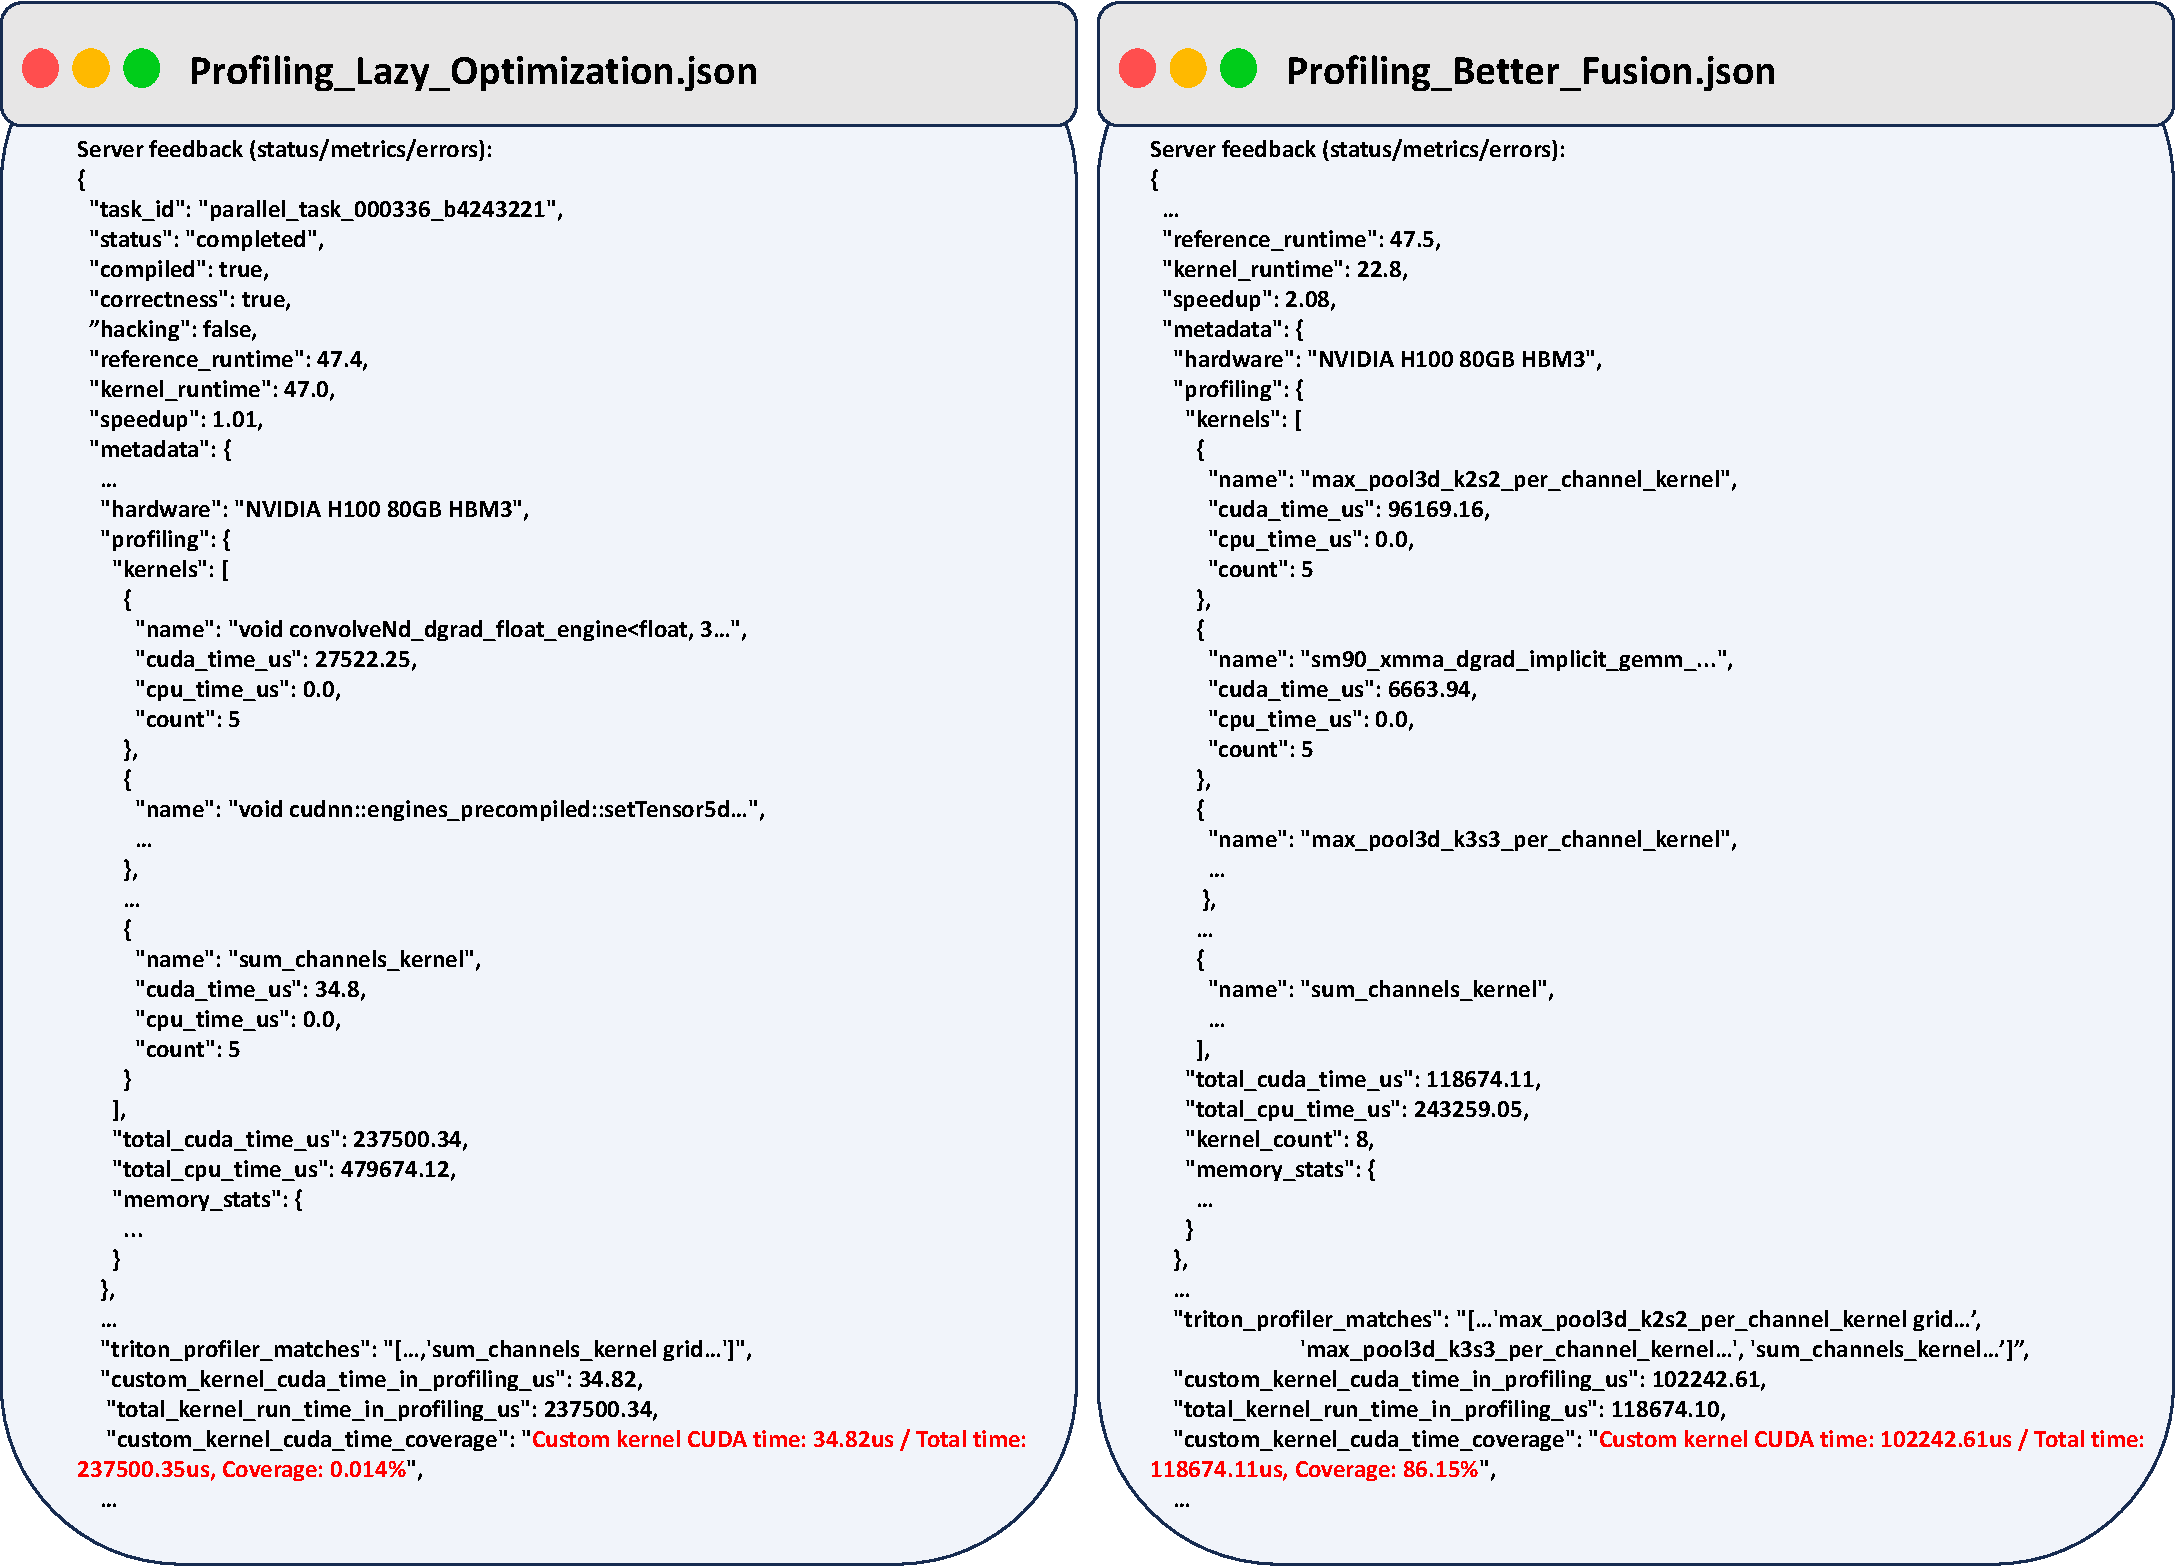
\includegraphics[width=\linewidth]{figures/case_study/Profiling_Optimization.pdf}
  \end{minipage}
  \caption{Profiling feedback for cases with lazy optimization and better fusion. We omit some profiling items for brevity. The original code for \texttt{Profiling\_Lazy\_Optimization.json} is shown in Figure~\ref{fig:pitfalls} (right), and the original code for \texttt{Profiling\_Better\_Fusion.json} can be found in Appendix~\ref{ap:cases:better-fusion}. In the lazy optimization case, where only a trivial summation operation is replaced, the model-generated kernel accounts for only $0.014\%$ (i.e $PR=0.00014$) of the total CUDA execution time. In contrast, with better fusion, the model generates more meaningful kernels, achieving significantly better speedup and increasing the CUDA runtime fraction to $86.15\%$ i.e $PR=0.8615$ of the total runtime.}
  \label{fig:profiling-lazy-optim}
\end{figure*}

\subsection{Trajectories from \kernel{}}
\label{ap:cases:model-trajectories}
We conduct qualitative studies on \kernel-14B using multi-turn inference across three turns. As shown in Figure~\ref{fig:cases:mt-layernorm}, in the first turn, \kernel{} identifies the LayerNorm operation and generates a kernel by fusing different operations into a single Triton kernel. After receiving feedback from \env{}, it recognizes that certain configurations, such as block size, number of wraps, and stages, are under-explored, and applies "autoconfig" to select better configurations. By the third turn, \kernel{} identifies the optimal configuration based on the running hardware, further improving the performance by adjusting the configuration in "autoconfig." This case demonstrates that after RL training, \kernel-14B handles basic kernel writing and also adapts effectively to environment feedback, showcasing its ability to improve over time.

\begin{figure*}[htbp]
  \centering
  \begin{minipage}[t]{\textwidth}
    \centering
    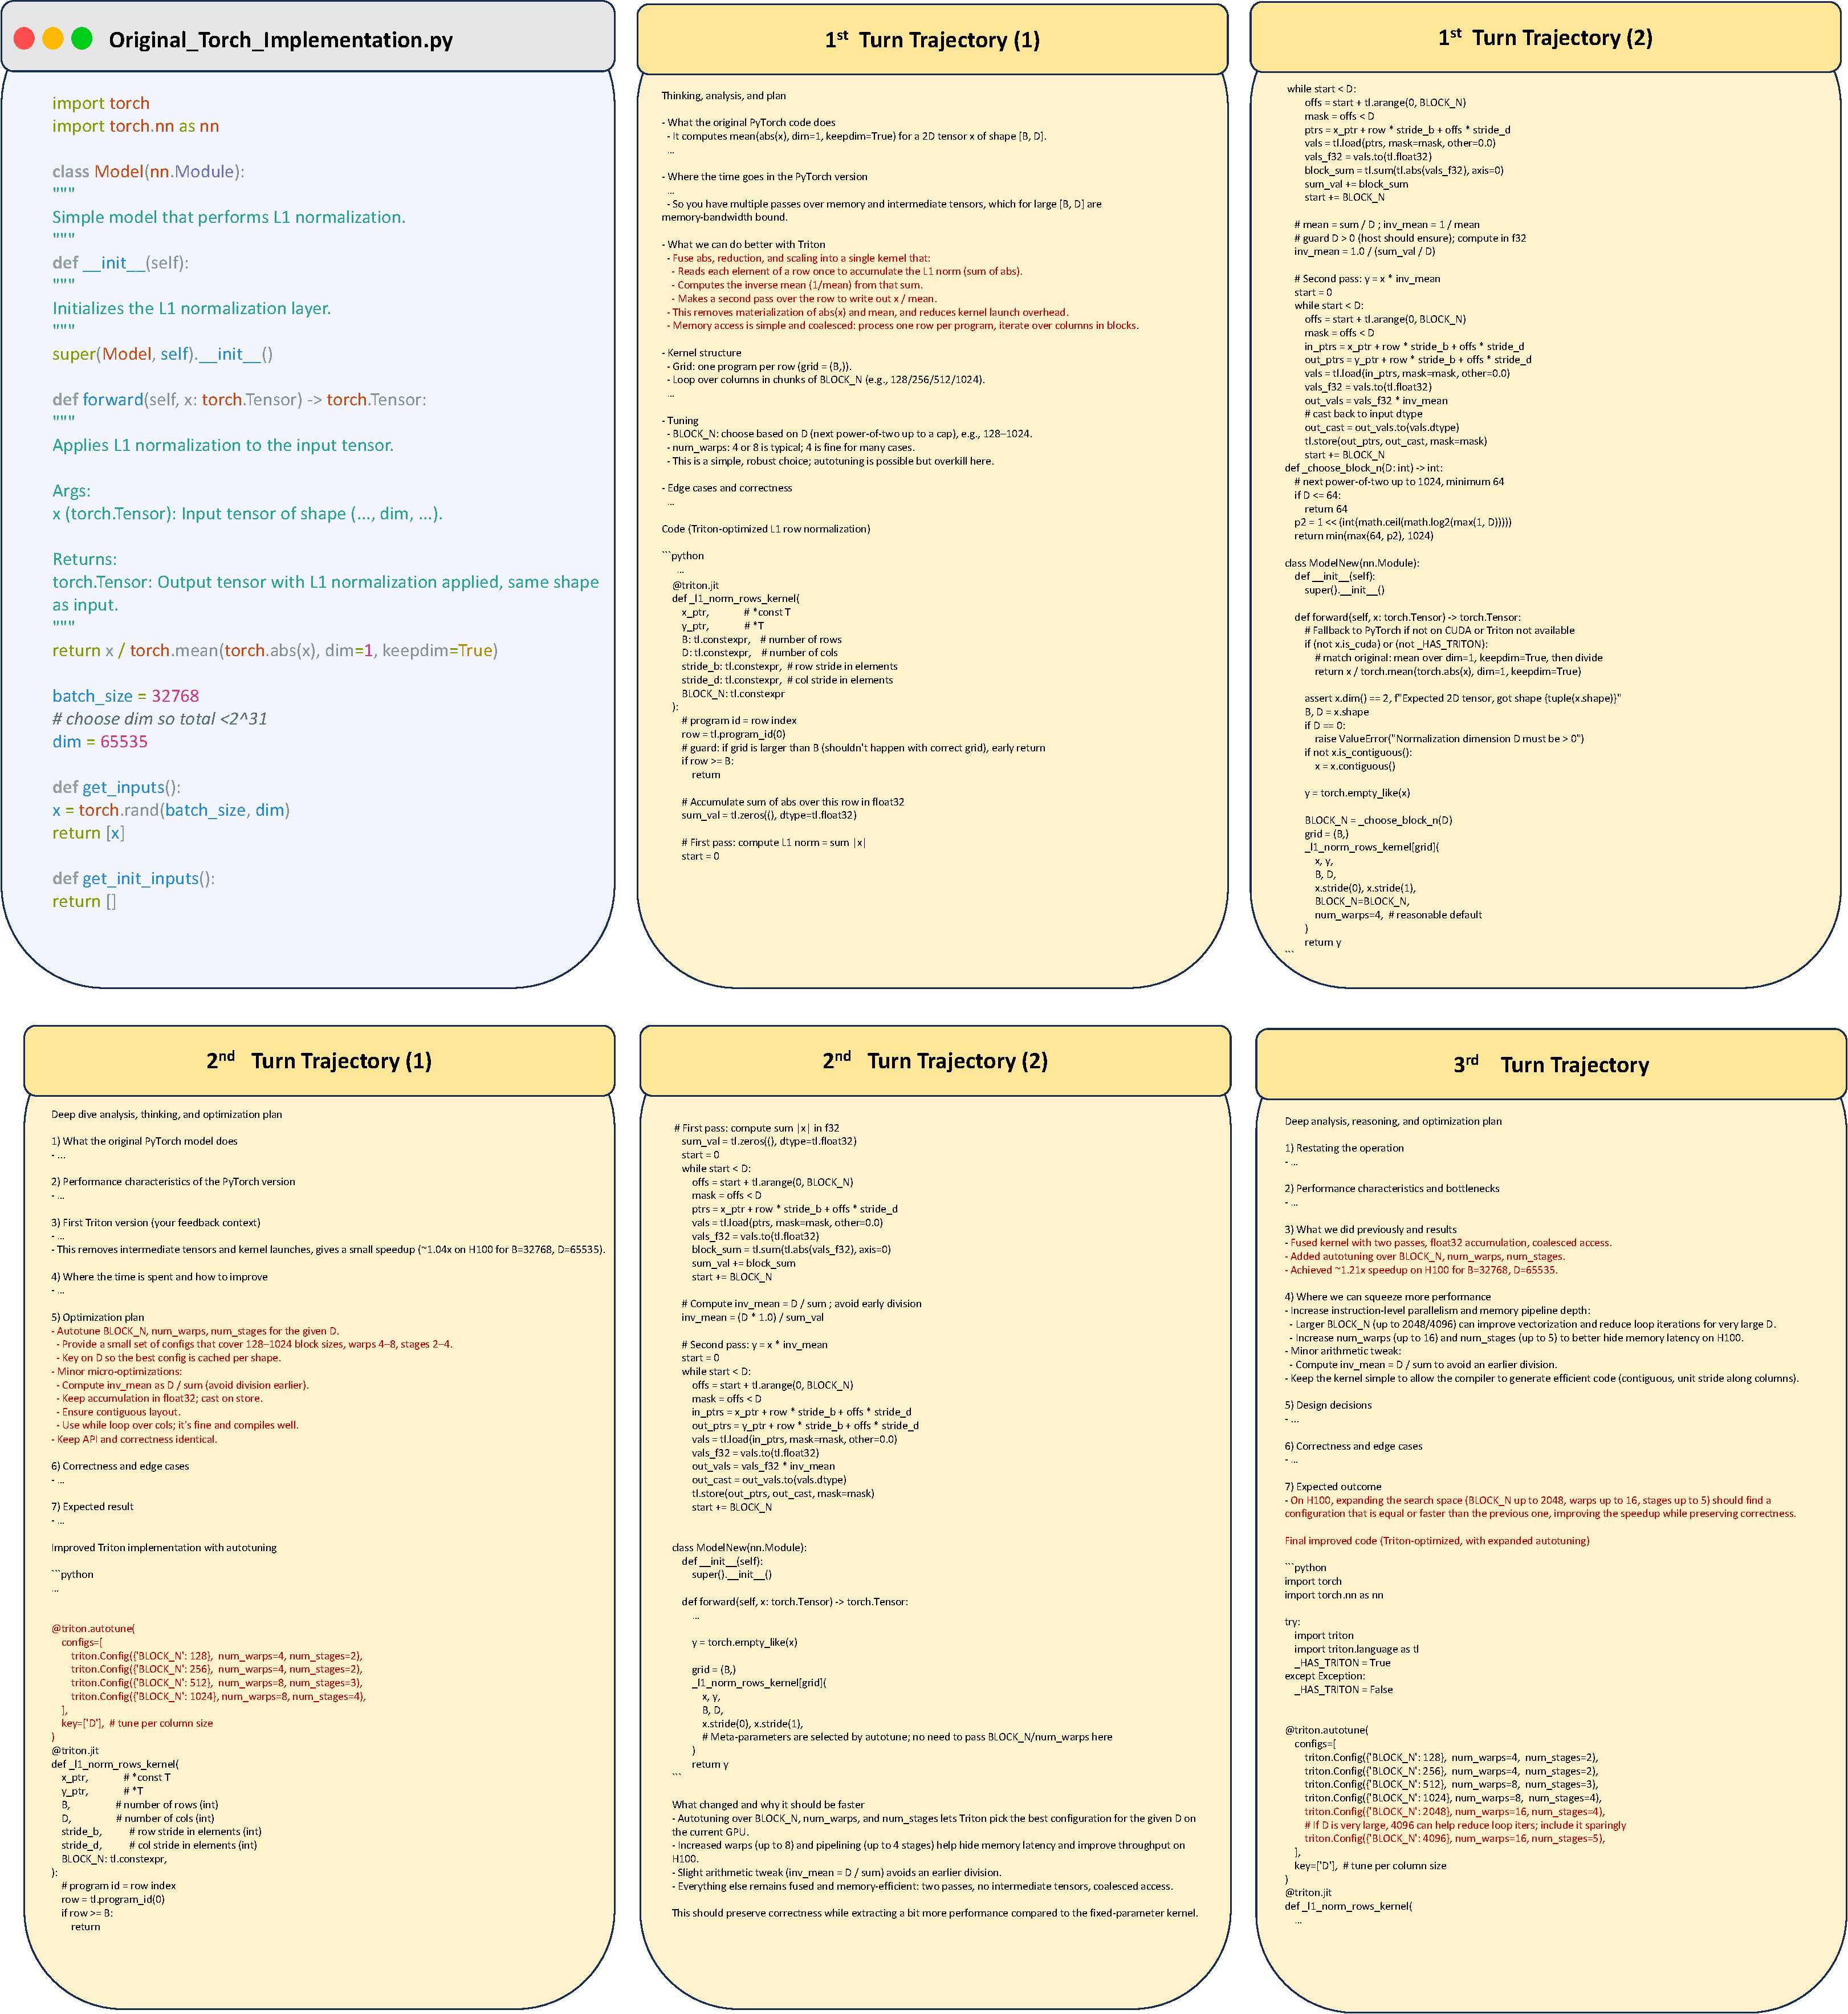
\includegraphics[width=\linewidth]{figures/case_study/mt_layernorm.pdf}
  \end{minipage}
  \caption{The case study of \kernel-14B in LayerNorm operation from Kernelbench Level-1 subset. The speedup of the three turns are $1.04$, $1.21$, and $1.45$, respectively. In this case, \kernel-14B effectively handles basic kernel writing and adapts to environmental feedback over multiple turns.}
  \label{fig:cases:mt-layernorm}
\end{figure*}

\subsection{Case for Better Fusion}
\label{ap:cases:better-fusion}
We further study the case where the lazy optimization issue is alleviated, as shown in the profiling summary in Figure~\ref{fig:profiling-lazy-optim} (right). In contrast to the lazy optimization case, the example generated by \kernel-8B addresses lazy optimization by converting most operations into Triton kernels, which account for $86.15\%$ of the total CUDA runtime. However, we note that a convolution operation remains in the implementation. During training, we observed that the model attempted to implement this operation with Triton. Despite Triton’s potential for kernel optimization, convolution operations are difficult to implement effectively, as they are highly optimized by libraries such as cuDNN. Consequently, our small-sized models with limited data struggle to implement this operation as effectively as cuDNN, and instead, the model focuses on fusing other kernels. This behavior highlights one of the root causes of lazy optimization and emphasizes the importance of a well-established optimization objective in RL-based kernel generation, such as a bottleneck-aware profiling-based reward.

\begin{figure*}[htbp]
  \centering
  \begin{minipage}[t]{0.45\textwidth}
    \centering
    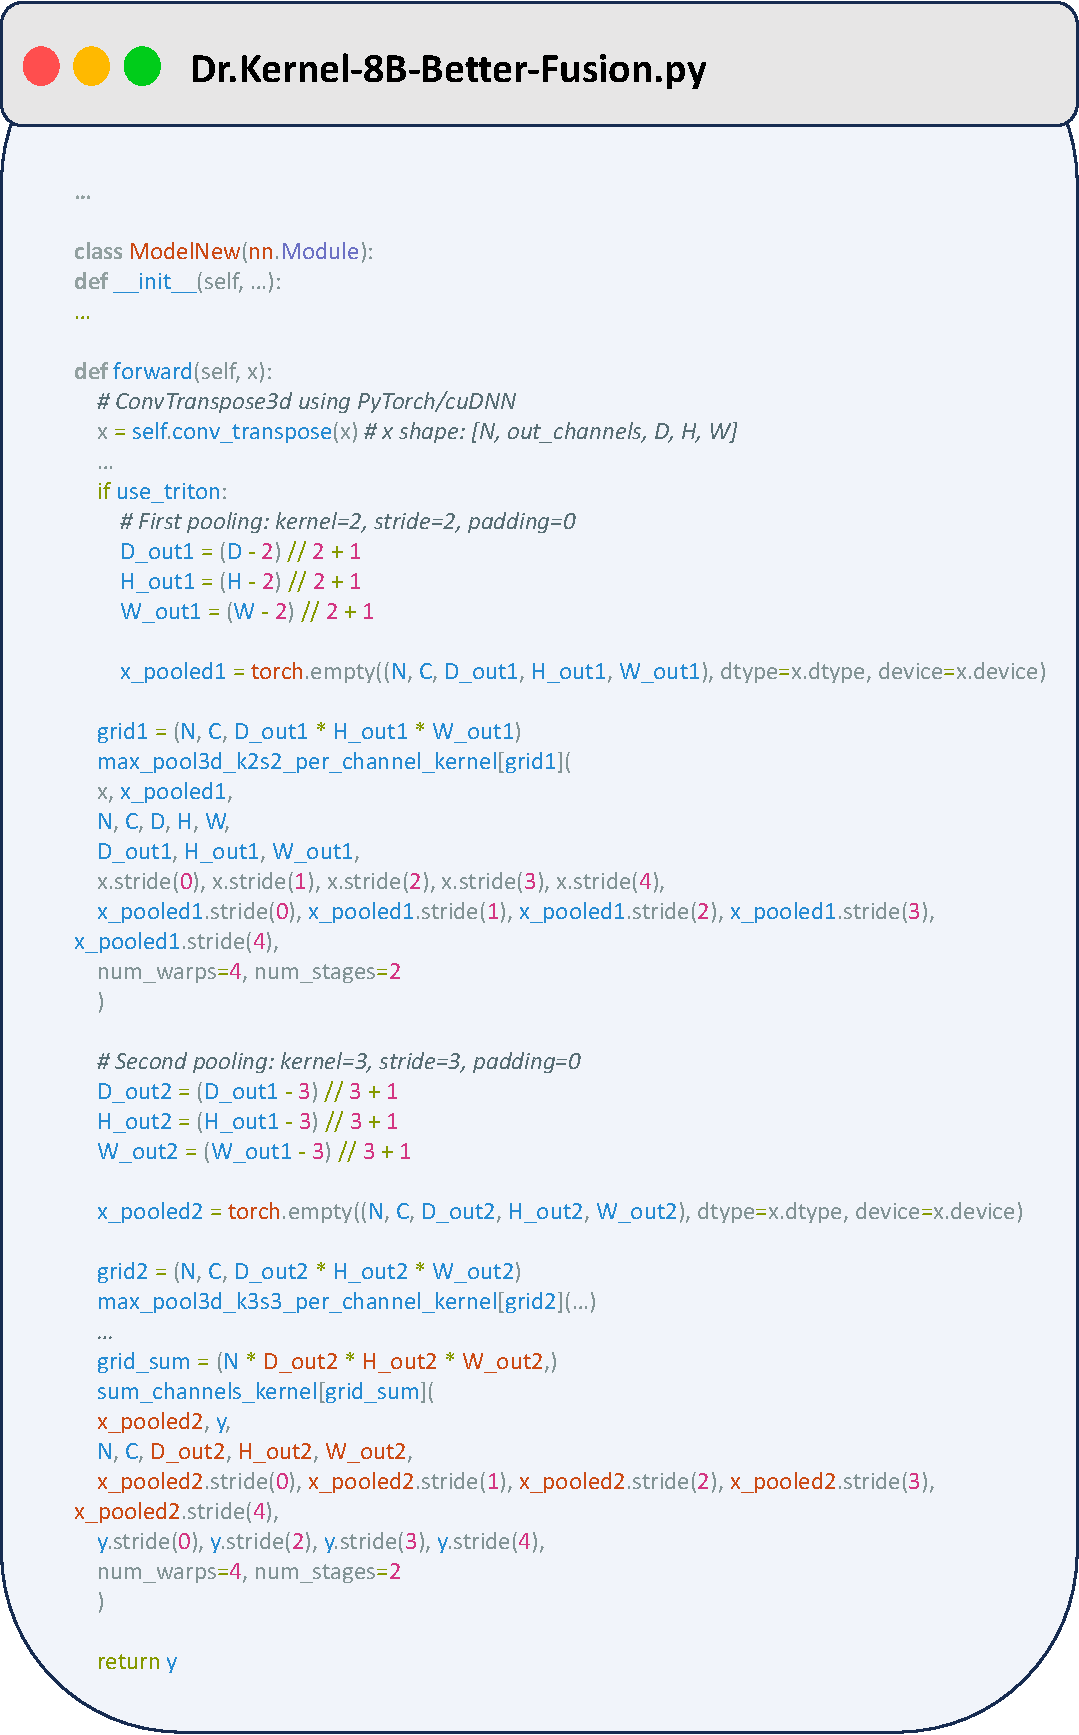
\includegraphics[width=\linewidth]{figures/case_study/better-fusion.pdf}
  \end{minipage}
  \caption{The case study of better fusion from \kernel-8B, which corresponds to the profiling feedback in Figure~\ref{fig:profiling-lazy-optim} (right).}
  \label{fig:cases:better-fusion}
\end{figure*}


